%!TEX TS-program = xelatex
%!TEX encoding = UTF-8 Unicode
\documentclass{icis}

\usepackage{graphicx}


\title{ICIS 2014 Auckland Paper Title}
\researchtype{Research in Progress}
\shorttitle{This is my test title}
\track{Human-computer Interaction}

\usepackage[authoryear,sort]{natbib}

\setcitestyle{aysep={}}

\begin{document}


\maketitle

\section{Introduction}

We ask that authors follow these basic guidelines when submitting to ICIS. In
essence, you should format your paper exactly like this document. The easiest
way to use this template is to replace the placeholder content with your own
material. The template file contains specially formatted styles (e.g.,
\texttt{Normal, Heading, Bullet, References, Title, Author, Affiliation}) that
are designed to reduce the work in formatting your final submission.

\section{Citations}

Citations should be done in the MISQ style. For direction, see the MISQ website
(http://www.misq.org/manuscript-guidelines), specifically the section on the
MISQ references format. Getting bibtex to do that is one goal of this
template. This is a test citation of a single author book
\citep{bonini_simulation_1963}, and a two author book section
\citep{chenhall_formal_1989}. Next comes the scary 4 author et
al. \citep{zhang2006}, and a multi-cite cite \citep{bonini_simulation_1963,
  ackoff_management_1961}. Check the references section at the end to see if
these are properly arranged.

\section{Page Size}
On each page, your material (not including the header and footer) should fit
within a rectangle of 18 x 23.5 cm (7 x 9.25 in.), centered on a US letter page,
beginning 1.9 cm (.75 in.) from the top of the page.  Please adhere to the US
letter size only (hopefully Word or other word processors can help you with
it). If you cannot do so, please contact the review coordinator for
assistance. All final publications will be formatted and displayed in US letter
size. Right margins should be justified, not ragged. All margins must measure 1"
(2.5 cm) around. Beware, especially when using this template on a Macintosh,
Word may change these dimensions in unexpected ways.

\section{Length}
Each type of submission (completed research papers, research-in-progress papers,
teaching cases, and panels) has specific page length requirements. See
additional requirements specific to each type of submission. Any submission that
exceeds page length limits will be rejected without review.

Completed research papers must not exceed fourteen (14) single-spaced pages. The
14 page count includes all text, figures, tables and appendices. Note that this
page count excludes the cover page, abstract, keywords and references. 

This paper length is intended to encourage authors to publish full-length papers
in journals or other outlets at a later date.

\section{Normal or Body Text}
Please use a 10-point Georgia font (similar to Times New Roman, but more easily
read online) or, if it is unavailable, another proportional font with serifs, as
close as possible in appearance to Times New Roman 10-point. On a Macintosh, the
similar font will be named Times and not Times New Roman. Please use sans-serif
or non-proportional fonts only for special purposes, such as source code text
(\texttt{\textbackslash texttt\{\}}). [References to Georgia font from this
point forward should be interpreted as ``Georgia or equivalent.'']

\section{Sections}
The heading of a section should be Georgia 13-point bold, left justified
(\texttt{\textbackslash section\{\}} in this template file).  Sections should not be numbered.

\subsection{Subsections}
Headings of subsections should be in Georgia 11-point bold italics with initial
letters capitalized (\texttt{\textbackslash subsection\{\}}). (Note: for
sub-sections and sub-subsections, words like 'the', 'of', 'a', 'an' are not
capitalized unless it is the first word of the heading.)

\subsubsection{Sub-subsections}
Headings for sub-subsections should be in Georgia 10-point bold with initial
letters capitalized (\texttt{\textbackslash subsubsection\{\}}). Please do not
go any further into another layer/level.

\section{Figures, Tables \& Captions}
Place figures and tables close to the relevant text (or where they are
referenced in the text).  Captions should be Georgia 10-point bold (Caption
Style in this template file).  They should be numbered (e.g., ``Table 1'' or
``Figure 2''), centered and placed beneath the figure or table.  Please note that
the words ``Figure'' and ``Table'' should be spelled out (e.g., ``Figure'' rather than
``Fig.'') wherever they occur. The proceedings will be made available online, thus
color figures are possible.

\subsection{Inserting Images}
Occasionally MS Word generates larger-than-necessary PDF files when images
inserted into the document are manipulated in MS Word. To minimize this
problem, use an image editing tool to resize the image at the appropriate
printing resolution (usually 300 dpi), and then insert the image into Word using
Insert | Picture | From File\ldots

As indicated in Figure 1, using tables to hold places can work very well in
Word. If you want to copy a figure from another application (such as PowerPoint)
and then paste to the place where you want your figure to be, make sure that (1)
the figure stays in the position, and (2) it does not take up too much
space. You can ensure the former by double clicking the figure, then go to
``Layout'' tab, and select ``In line with text.'' To ensure the latter, use ``Paste
Special,'' then select ``Picture.'' You can resize the figure to your desired size
once it is pasted. Look at Figure~\ref{fig:test}.

% Test image
\begin{figure}[h]
  \centering
  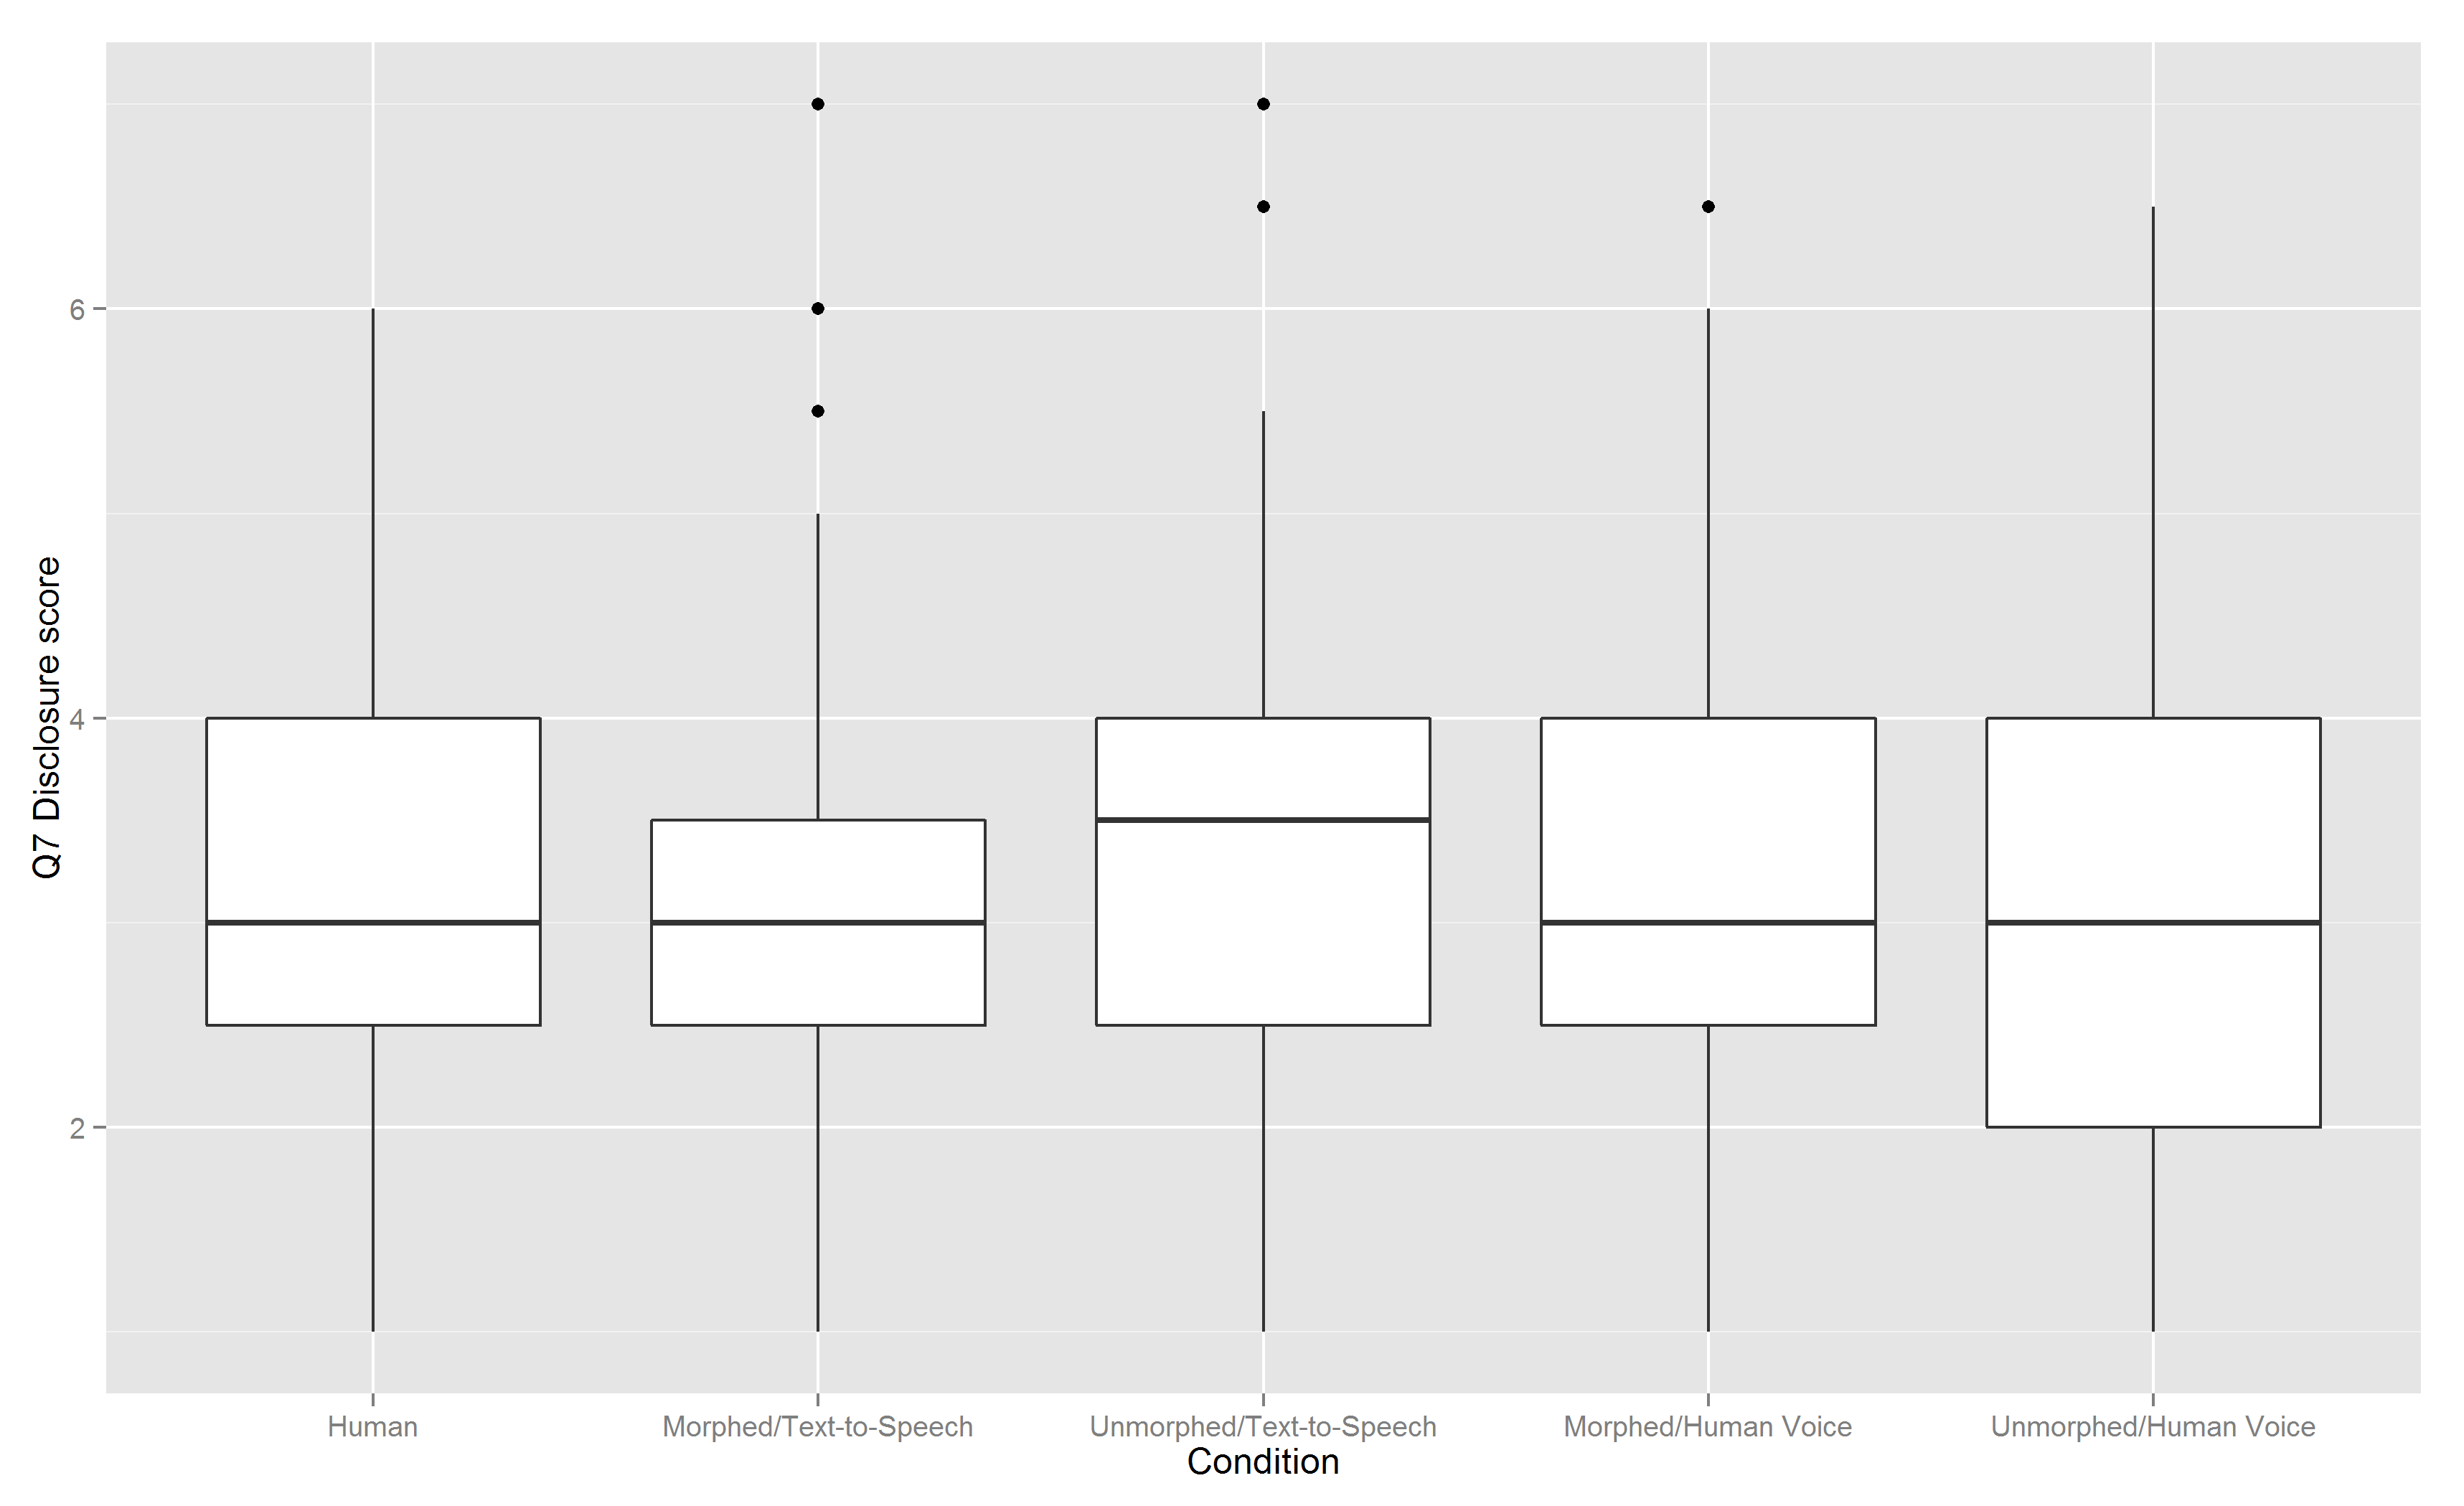
\includegraphics[scale = 0.45]{testimage.png}
  \caption{Sample caption. Should be bold, centered, and below} 
  \label{fig:test}
\end{figure}


\subsection{Table Style}
Inserting a table in the text can work well. You may want to adjust the vertical
spacing of the text in the tables. (In Word, use Format | Paragraph\ldots~and
then the Line and Page Breaks tab. Generally, text in each field of a table will
look better if it has equal amounts of spacing above and below it, as in
Table~\ref{tab:lme-mean}.)

This is what a test table might look like. 

\begin{table}[ht]
\centering
\begin{tabular}{rrrrrr}
  \hline
 & Value & Std.Error & DF & t-value & p-value \\ 
  \hline
(Intercept) & 1276.635 & 49.538 & 557.000 & 25.771 & 0.000 \\ 
  condition & 11.870 & 65.694 & 49.000 & 0.181 & 0.857 \\ 
  valence & 207.347 & 55.009 & 557.000 & 3.769 & 0.000 \\ 
  deception & -40.372 & 63.519 & 557.000 & -0.636 & 0.525 \\ 
   \hline
\end{tabular}
\caption{Test table with caption} 
\label{tab:lme-mean}
\end{table}

\section{Language, Style, and Content}
With regard to spelling and punctuation, you may use any dialect of English
(e.g., British, Canadian, US, etc.) provided this is done
consistently. Hyphenation is optional. To ensure suitability for an
international audience, please pay attention to the following:

\begin{itemize}
\item Write in a straightforward style.
\item Try to avoid long or complex sentence structures.
\item Briefly define or explain all technical terms that may be unfamiliar to
  readers.
\item Explain all acronyms the first time they are used in your text - e.g.,
  ``primary care provider (PCP)''.
\item Explain local references (e.g., not everyone knows all city names in a
  particular country).
\item Be careful with the use of gender-specific pronouns (he, she) and other
  gendered words (chairman, manpower, man-months). Use inclusive language that
  is gender-neutral (e.g., they, s/he, chair, staff, staff-hours, person-years).
\end{itemize}

\bibliographystyle{misq}
\bibliography{references}

\end{document}